\documentclass{article}

% Math
\usepackage{amsmath,amssymb,amsthm,mathtools}
\usepackage{physics}       % \grad, \div, \laplacian, \pd, etc.

% Units
\usepackage{siunitx}
\sisetup{per-mode=symbol, detect-all}

% Graphics & diagrams
\usepackage{graphicx}
\usepackage{grffile}

% Theorems / definitions
\theoremstyle{definition}
\newtheorem{definition}{Definition}[section]
\theoremstyle{plain}
\newtheorem{theorem}{Theorem}[section]
\theoremstyle{remark}
\newtheorem{remark}{Remark}[section]

% Useful short commands for EM notes
\newcommand{\E}{\mathbf{E}}
\newcommand{\B}{\mathbf{B}}

\begin{document}

\section*{The Electric Field}
The force that affects charged particles was found to be similar to the force of gravity in many ways.
As it depends on a common quantity between both bodies, that quantity is mass in the case of gravity and charge in the case of the electric force, and on the squared distance between them.
This can be represented by the very famous Coulomb's law:

\begin{equation}
    \bar{F} = \frac{q_1 q_2}{4\pi \epsilon_0 r^2} \hat{r}
    \label{eq.Coulomb}
\end{equation}
\\
Where $\epsilon_0$ is the permittivity of free space (how much it allows electric forces).\medskip

The main difference between both forces is that gravity is always an attracting force,
however, the electric force can attract or repel depending on the charges of the bodies.

Besides the forces between two charges, it's also important to look at the effect of electric charges on the space around them;
In that case we can't use Coulomb's law, since it depends one two charges. We should look at the effect of our isolated charge on a unit charge anywhere around it,
that effect is called \textit{the electric field}.

\begin{figure}[htbp]
    \centering
    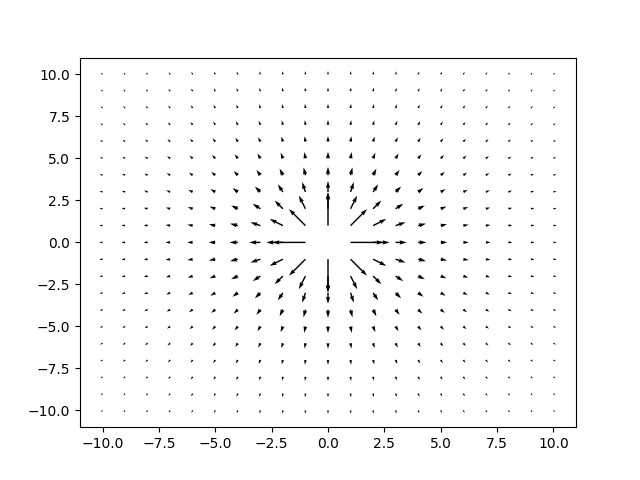
\includegraphics[width=0.8\textwidth]{Media/Graphs/Point.png}
    \caption{Electric field of a point charge.}
    \label{fig.point-field}
\end{figure}

So if we place a unit charge at every point in space and measure the force acting on it then we can understand the effect of the electric charges on free space.
Based on that, the following definition for the electric field should be very straightforward.

\begin{definition}
    The effect of electric charges on any point in space can be represented by a vector field of the force applied by these charges on a unit charge at that point in space,
    that vector field is called an \textit{electric field}.
    The force exerted by a point charge on a unit charge can be calculated by making a minor change to \textbf{Eq. \ref{eq.Coulomb}}.
    \begin{equation}
        \bar{E} = \frac{q}{4\pi \epsilon_0 r^2} \hat{r}
    \end{equation}
\end{definition}



\section*{Electric Potential}
When a body is thrown into the air, it losses more kinetic energy the higher it goes. We can interpret this, knowing that the body can regain its kinetic energy,
as the body storing kinetic energy in the form of a new type of energy called \textit{potential energy}. We can be sure that the energy can be regained since we know that
gravity generates a field which locally looks like this:
\begin{center}
    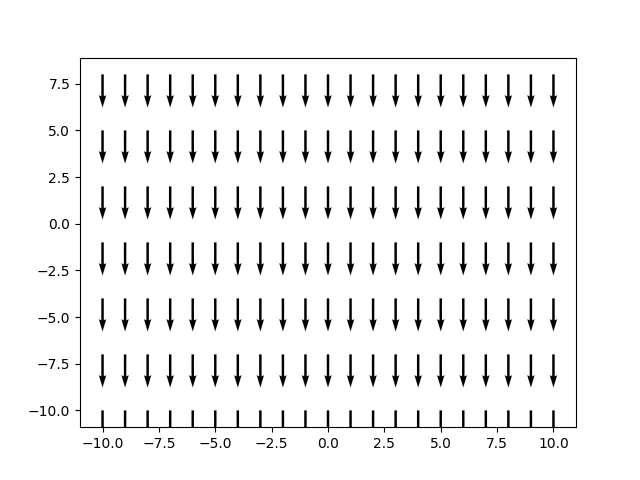
\includegraphics[width=0.8\textwidth]{Media/Graphs/Gravity.png}
\end{center}

For this field, the energy lost as the body goes up is stored, then regained as it goes down.
The difference of potential energy between two points is the amount taken away from the body's kinetic energy to be stored by the field.
So when the work done by the field is negative the stored potential energy increases.

\begin{definition}
    The \textit{potential energy difference} between two points $a$ and $b$ in a conservative force field $\bar{F}$ is defined as
    $$
        U(b) - U(a) = -W_{field} = - \int_a^b \bar{F} \cdot d\bar{l}
    $$
    where $U$ is the potential energy.
\end{definition}

We can pick a reference point $o$ and assign it an absolute potential energy of zero,
then the potential energy of any other point $A$ would be the energy stored as the body moves from $o$ to $A$.

\begin{definition}
    The \textit{absolute potential energy} at a point $A$ is the potential energy difference between $A$ and the reference point.
    $$
    U(A) = - \int_o^A \bar{F} \cdot d\bar{l}
    $$
\end{definition}

These concepts can be generalised to any \textit{conservative} force field, in our case the most relevant is the electric field.
The reader can look back at \textbf{figure \ref{fig.point-field}} to imagine how the electric field can conserve energy.

When we try to apply this definition to electric forces we'll come across a problem,
since the electric force depends on the charges which it affects we can't assign an \underline{absolute} potential energy to a point in space, the potential energy would still depend on the body's charge.
So in the next definition we'll use the electric field instead of the electric force, and assign every point in space the value of the stored energy of a unit charge at that point.

\begin{definition}[The Electric Potential]
    The \textit{electric potential difference} between two points $a$ and $b$ in an electric field $\bar{E}$ is defined as
    $$
        V(b) - V(a) = - \int_a^b \bar{E} \cdot d\bar{l}
    $$

    And the \textit{absolute electric potential} at a point $A$ is the electric potential difference between $A$ and the reference point $o$.
    $$
    V(A) = - \int_o^A \bar{E} \cdot d\bar{l}
    $$
\end{definition}
\end{document}